\documentclass[11pt]{article}
\usepackage[left=2cm,top=2cm,right=2cm,bottom=2cm]{geometry}
\usepackage{graphicx}
\usepackage{setspace}
\usepackage{caption}
\usepackage{subcaption}
\usepackage{amsmath}
\usepackage{amsthm}
\usepackage[]{algorithm2e}
\usepackage{amsmath}
\usepackage[noend]{algpseudocode}
\usepackage{float}
\title{COMP 440 Homework 2}
\author{Tony Chen(xc12) and Adam Wang(sw33)}
\date{September 2016}
\begin{document}
\begin{onehalfspace}
\section{Pursuit evasion games}
 \renewcommand{\theenumi}{\alph{enumi}}
    \begin{enumerate}
    \item Copy of game tree, with terminal utility denoted:\\
     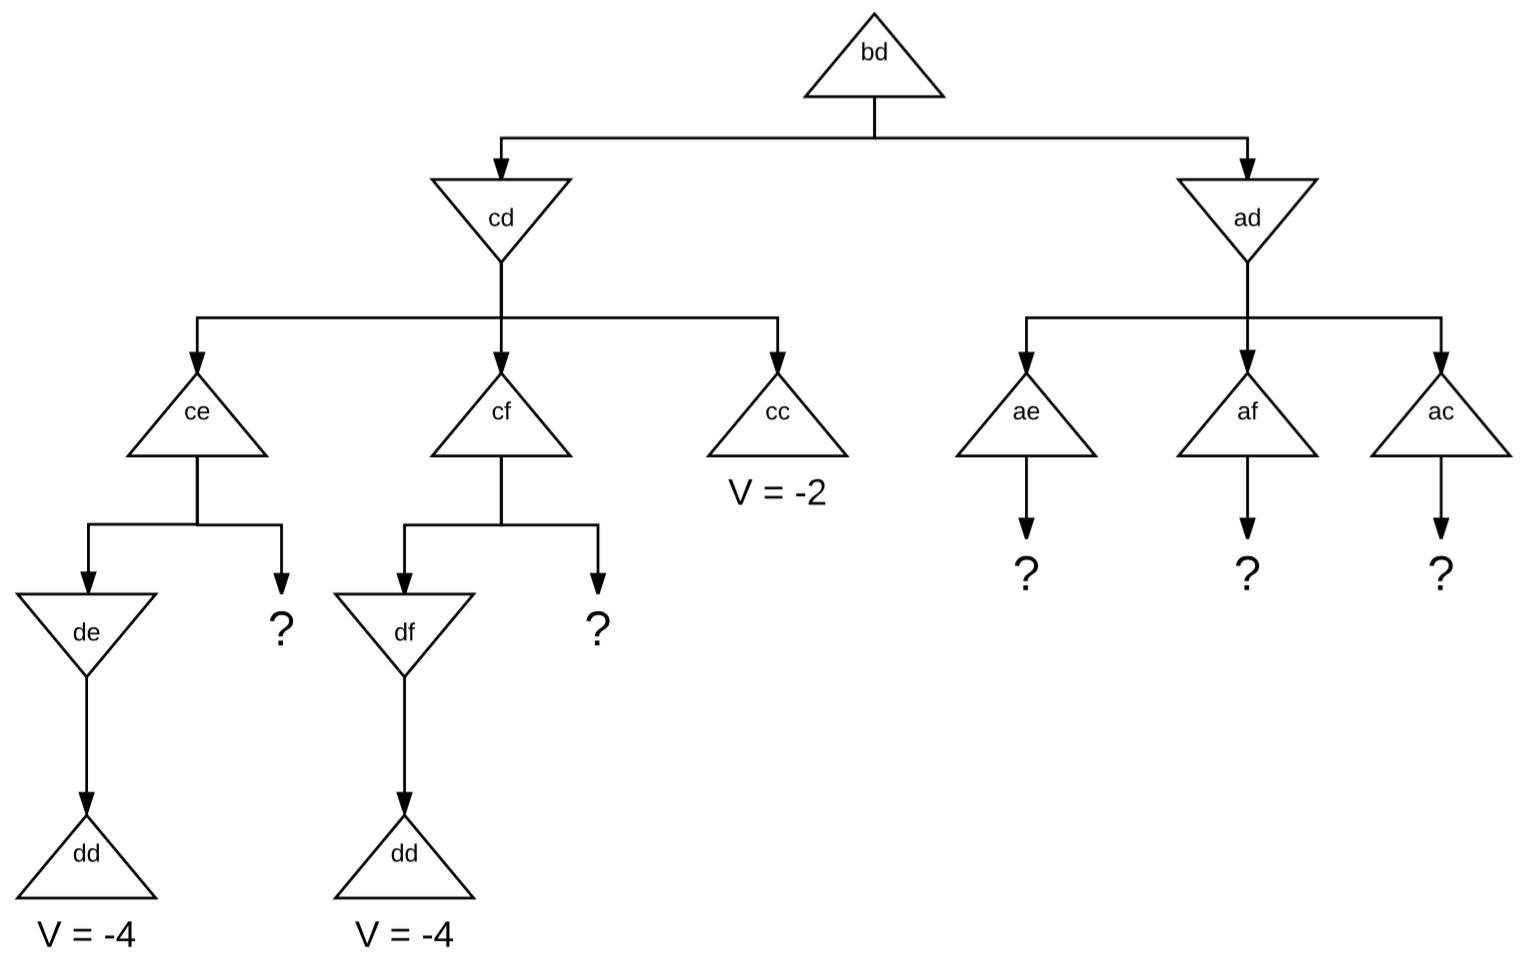
\includegraphics[width=16cm, height=9cm]{1_a.png}\\
     \item The inference of each internal node's value is labeled:\\
     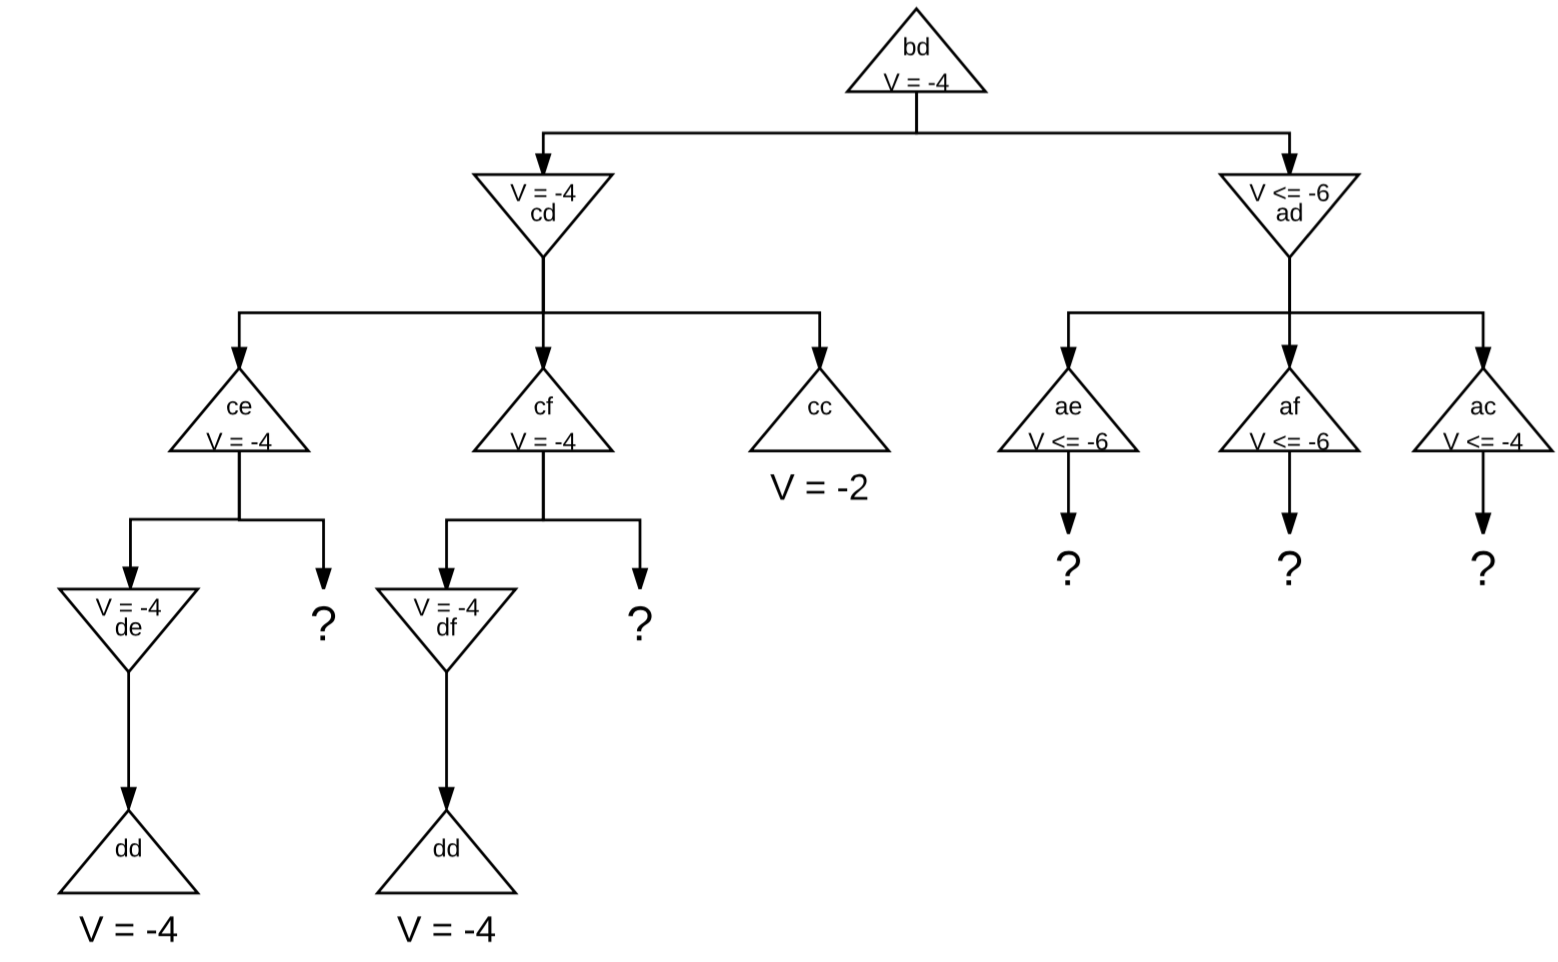
\includegraphics[width=16cm, height=9cm]{1_b.png}\\
     \item Name added:\\
     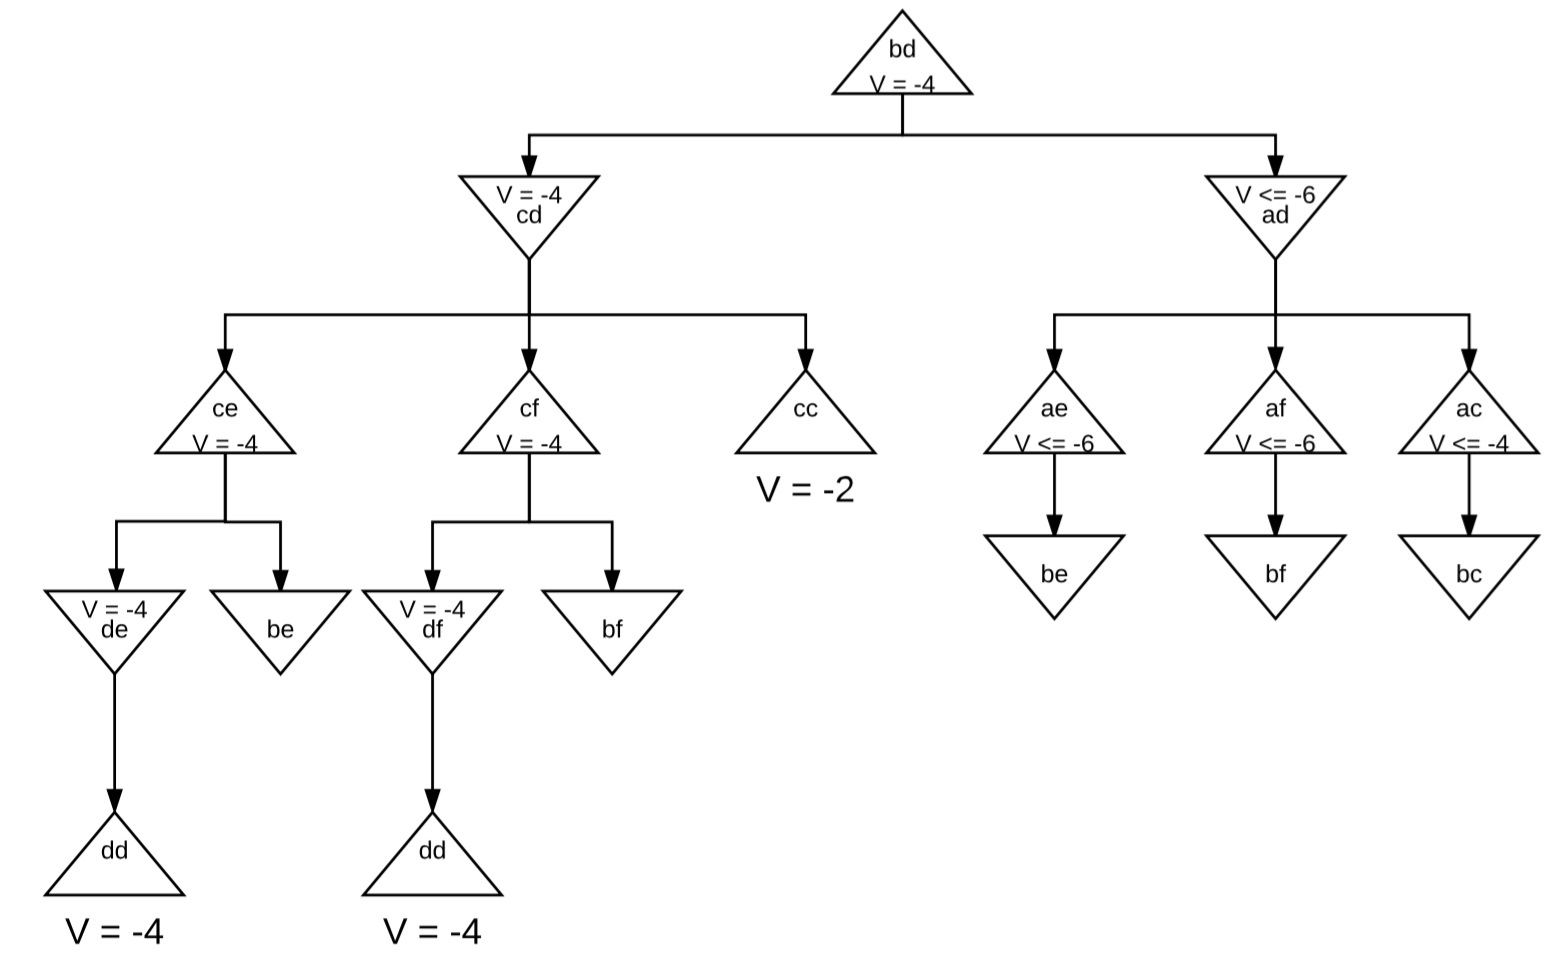
\includegraphics[width=16cm, height=9cm]{1_c.png}\\
     \item
     For a given internal node $PE$, an upper bound of its value is the negative of sum of 1) the cost so far to reach this node (i.e. the path sum from it to the root) and 2) the shortest path between $P$ and $E$. For the negative sum, the former cost has already occurred as a truth, and the latter must not be an overestimate, so their negative sum gives the upper bound. Following this conclusion, we can get bounds as following: $V(cd) <= -(1+1) = -2$, $V(ce) <= -(2+2) = -4$, $V(de) <= -(3+1) = -4$, $V(cf) <= -(2+2) = -4$, $V(df) <= -(3+1) = -4$, $V(ad) <= -(1+3) = -4$, $V(ae) <= -(2+4) = -6$, $V(af) <= -(2+4) = -6$, $V(ac) <= -(2+2) = -4$\\
     For the new nodes in (c), the bounds are: $V(be) = -(3+3) = -6$, $V(bf) = -(3+3) = -6$, $V(be) = -(3+3) = -6$, $V(bf) = -(3+3) = -6$, and $V(bc) = -(3+1) = -4$\\
     Note that, however, the bounds based on shortest-path is loose since it expects the Evader to "cooperate", which will not happen in a standard setting. So in part(b) the values for some of those internal nodes are much tighter.\\
     \item $be$ need not to be expanded because we already got $-4$ from $de$ (maximum here), and after we got $V(df) = -4$, we don't need to consider $bf$ because if it's larger than $-4$ then $cf$ will be larger than $-4$ and $cd$ will still take minimum ($-4$) from $ce$; if it's smaller than $-4$ then $cf$ will take $-4$ from $df$. $be$ will not be expanded because $bd$ will take the maximum between $cd$ ($-4$) and $ad$, and since $ad$ will take the minimum of $ae$, $af$, and $ac$, $bf$ and $bc$ will not even be considered (the value up to $-6$ at $ae$ already capped $ad$ from being chosen by $bd$ over $cd$).\\
     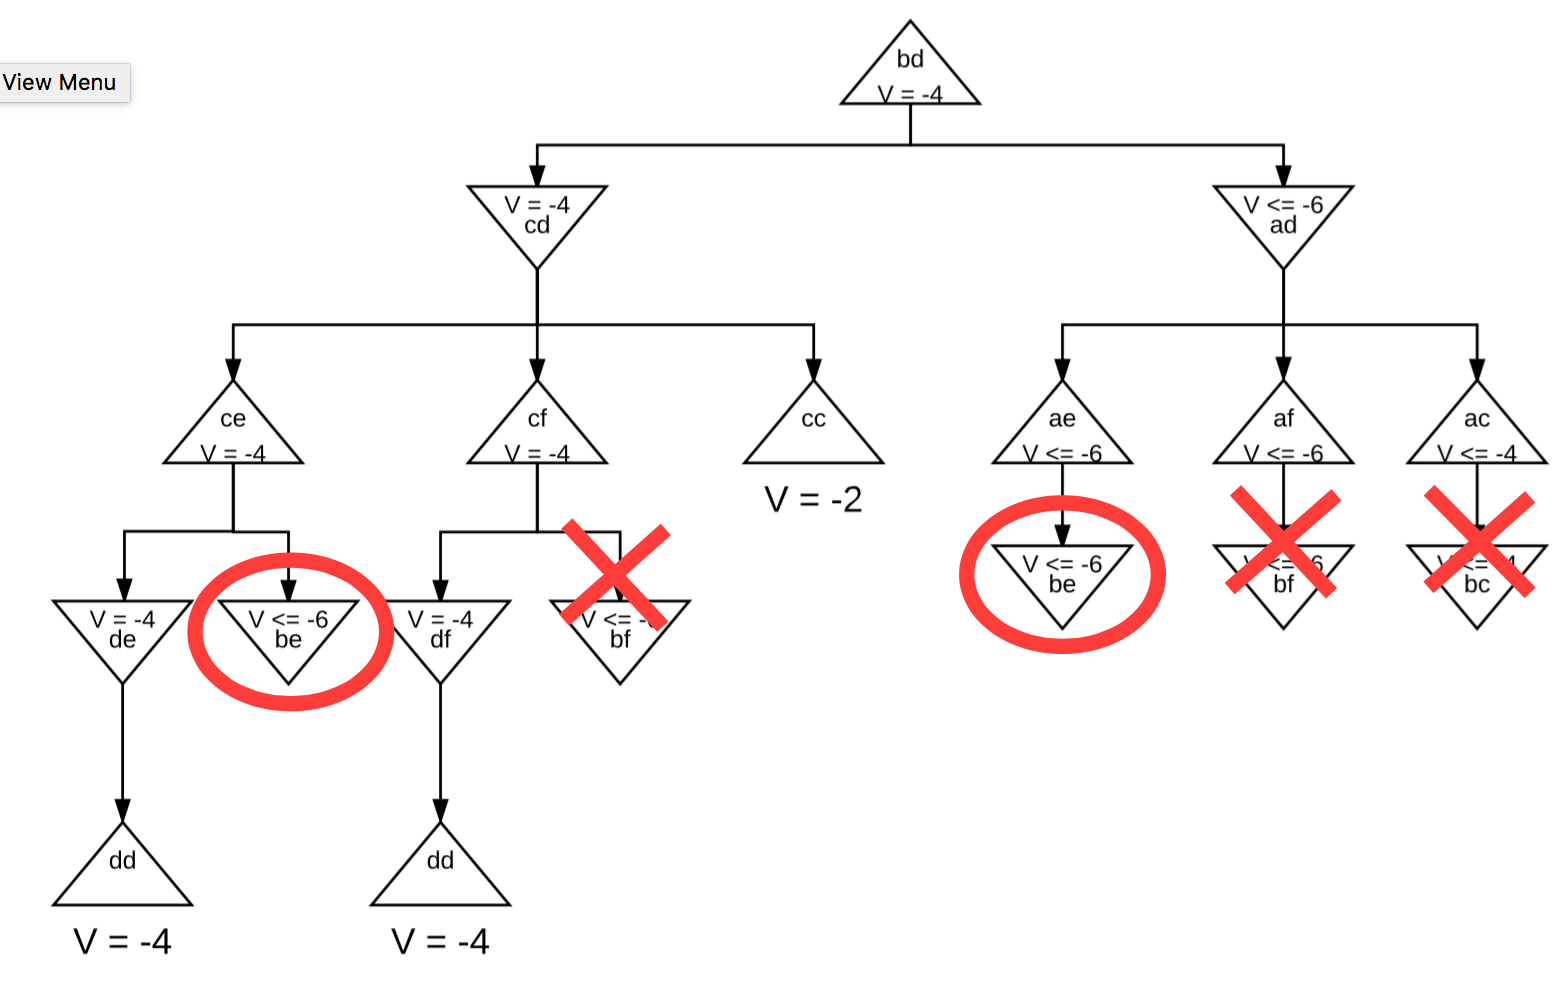
\includegraphics[width=16cm, height=9cm]{1_e.png}\\
     \item
     If the tree is finite, then the Pursuer will always win. This can be proved recursively:\\
     Initially, move the Pursuer up until it's at the lowest common ancestor node of P and E (this can always be achieved in finite steps since the Pursuer can always move up to the root of the entire tree).\\
     Consider the subtree whose root is the node where the Pursuer is. \\
     Base case: there is only one node in the subtree, in which case both the Pursuer and the Evader are on that node and the Pursuer catches the Evader.\\
     Recursive case: if the Evader is also on this root then the Pursuer already catches the Evader. Otherwise move the Pursuer down to the subtree child that contains the Evader.\\
    \end{enumerate}
\section{Minimax and expectimax}
\begin{itemize}
\item The values outside the parentheses are minimax, and the values inside the parentheses are expectimax:\\
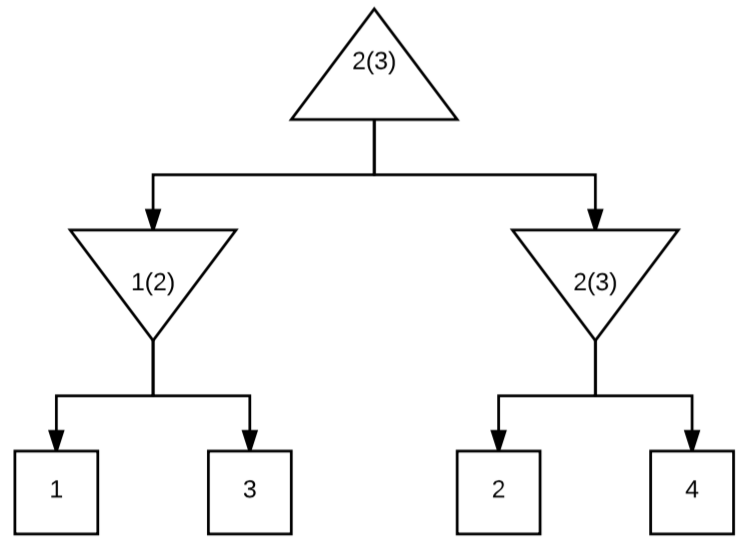
\includegraphics[width=12cm, height=9cm]{2_1.png}\\
\item
It is not possible.\\
Consider any Player 2 node $s_0$ and all of its children nodes $s_1,s_2,...,s_n$. For minimax we have $V_{min}(s_0) = Min(V(s_1), V(s_2), ..., V(s_n))$; for expectimax we have $V_{exp}(s_0) = Avg(V(s_1), V(s_2), ..., V(s_n)) \leq Min(V(s_1), V(s_2), ..., V(s_n)) = V_{min}(s_0)$. So it is not possible for a root node to have a larger value by minimax than by expectimax.\\
\item
Assumption: Player 2 is a perfect player that makes the best possible move every turn\\
\item
Assumption: Player 2 is a stochastic player whose moves can be described by some statistical distribution.\\
\item
1. Preprocess: Go through the game tree by substituting all Player 1 nodes (max nodes) with uniform chance nodes and record which child node Player 2 will pick at each min node.\\
2. Actual play: Go through the game tree with the knowledge of which child node Player 2 will pick at each node. Essentially Player 2 nodes are no longer min nodes but nodes the follow the outcome policy of the preprocess.\\
\end{itemize}
\section{Multi-agent pacman}
\subsection{Warmup}
\subsection{Problem 1: Minimax}
\begin{itemize}
\item
Assuming $isEnd(s)$ also returns $True$ if $depth(s) = 0$:
\[
    V_{opt}(s)=
    \begin{cases}
    Evaluation(s) & \text{if } isEnd(s)\\
    Max(V_{opt}(Successor)\: \forall \: Successor \in Actions(s)) & \text{if NOT } isEnd(s) \text{ AND } Player(s) \text{ is } a_0\\ 
    Min(V_{opt}(Successor)\: \forall \: Successor \in Actions(s)) & \text{Otherwise}
    \end{cases}
\]
\end{itemize}
\subsubsection{Observations}
\begin{itemize}
\item
The reason that pacman thrash around right next to a dot is that the Minimax depth is so small that pacman does not know what to do after eating the dot.\\
\item
Since pacman applies Minimax policy, in this case either going left or right will result in death, so he wants to die as soon as possible since there is a time penalty and dying sooner will result in a relatively higher score.\\
\end{itemize}
\subsection{Problem 2: Alpha-beta pruning}
\subsection{Problem 3: Expectimax}
\begin{itemize}
\item
Assuming $isEnd(s)$ also returns $True$ if $depth(s) = 0$:
\[
    V_{opt,\pi}(s)=
    \begin{cases}
    Evaluation(s) & \text{if } isEnd(s)\\
    Max(V_{opt,\pi}(Successor)\: \forall \: Successor \in Actions(s)) & \text{if NOT } isEnd(s) \text{ AND } Player(s) \text{ is } a_0\\ 
    \frac{\sum(V_{opt,\pi}(Successor)\: \forall \: Successor \in Actions(s))}{Len(Actions(s))} & \text{Otherwise}
    \end{cases}
\]
\item
In the trappedClassic case, since pacman applies Expectimax now, instead of thinking both ways are dead ends, he'd see now that going left would have a chance of winning since he knows ghost agents are random (i.e. not optimal) while going right would still be a sure way to die. So now his decision is different from its Minimax version.\\

\end{itemize}
\end{onehalfspace}
\end{document}